\chapter{Proposed Approach and Methodology}\label{chap:5}
\label{chap:approach}
\noindent This chapter presents the methodology through which the proposed Network Intrusion Detection and Prevention System (NIDPS) detects and blocks malicious traffic on a small network. The proposed approach is a hybrid detection framework: three complementary detection layers, a decision-fusion algorithm that turns their outputs into a single verdict, and an enforcement and recovery mechanism that acts on that verdict. The chapter begins with the datasets and the way they are harmonised so that models trained offline see the same features at runtime. It then walks through the backend algorithms that are not visible in the system design: flow construction, TLS fingerprinting, rule-based detection, Isolation Forest scoring with per-network threshold calibration, supervised attack classification, verdict fusion, automated blocking and the failure-handling state machine. The chapter closes with the evaluation protocol used to measure detection quality and the behaviour of the system on constrained hardware.

\section{Overview of the Proposed Framework}\label{sec:5.1}
\label{sec:overview}
\noindent The NIDPS runs on a single Linux host that acts as the network's wireless access point, so every packet between client devices and the ISP gateway passes through it. Each packet travels two paths at once. On the inline path, Suricata inspects packets as they are forwarded and can drop them immediately. On the analysis path, packets are grouped into bidirectional flows, and each completed flow is described by 78 statistical features plus TLS fingerprints (JA3/JA3S). These flow records are scored by an unsupervised Isolation Forest (Layer~2) and a supervised Random Forest/XGBoost classifier (Layer~3).

\noindent The three layers cover different threat classes:
\begin{itemize}
    \item \textbf{Layer 1 -- Signature detection (Suricata):} known attacks with stable signatures, such as SSH brute force, port scanning and DNS spoofing.
    \item \textbf{Layer 2 -- Anomaly detection (Isolation Forest):} traffic that deviates from the network's normal profile, including zero-day behaviour, C2 beaconing and data exfiltration.
    \item \textbf{Layer 3 -- Supervised classification (Random Forest/XGBoost):} assignment of suspicious flows to known attack families such as DDoS and lateral movement.
\end{itemize}

\noindent A decision-fusion engine combines the three outputs into one verdict per flow (pass, alert or block). Block verdicts are enforced through iptables and ipset. A watchdog supervises every component and applies the configured failure mode when one of them stops. Figure~\ref{fig:pipeline} summarises this pipeline.

\begin{figure}[!htbp]
    \centering
    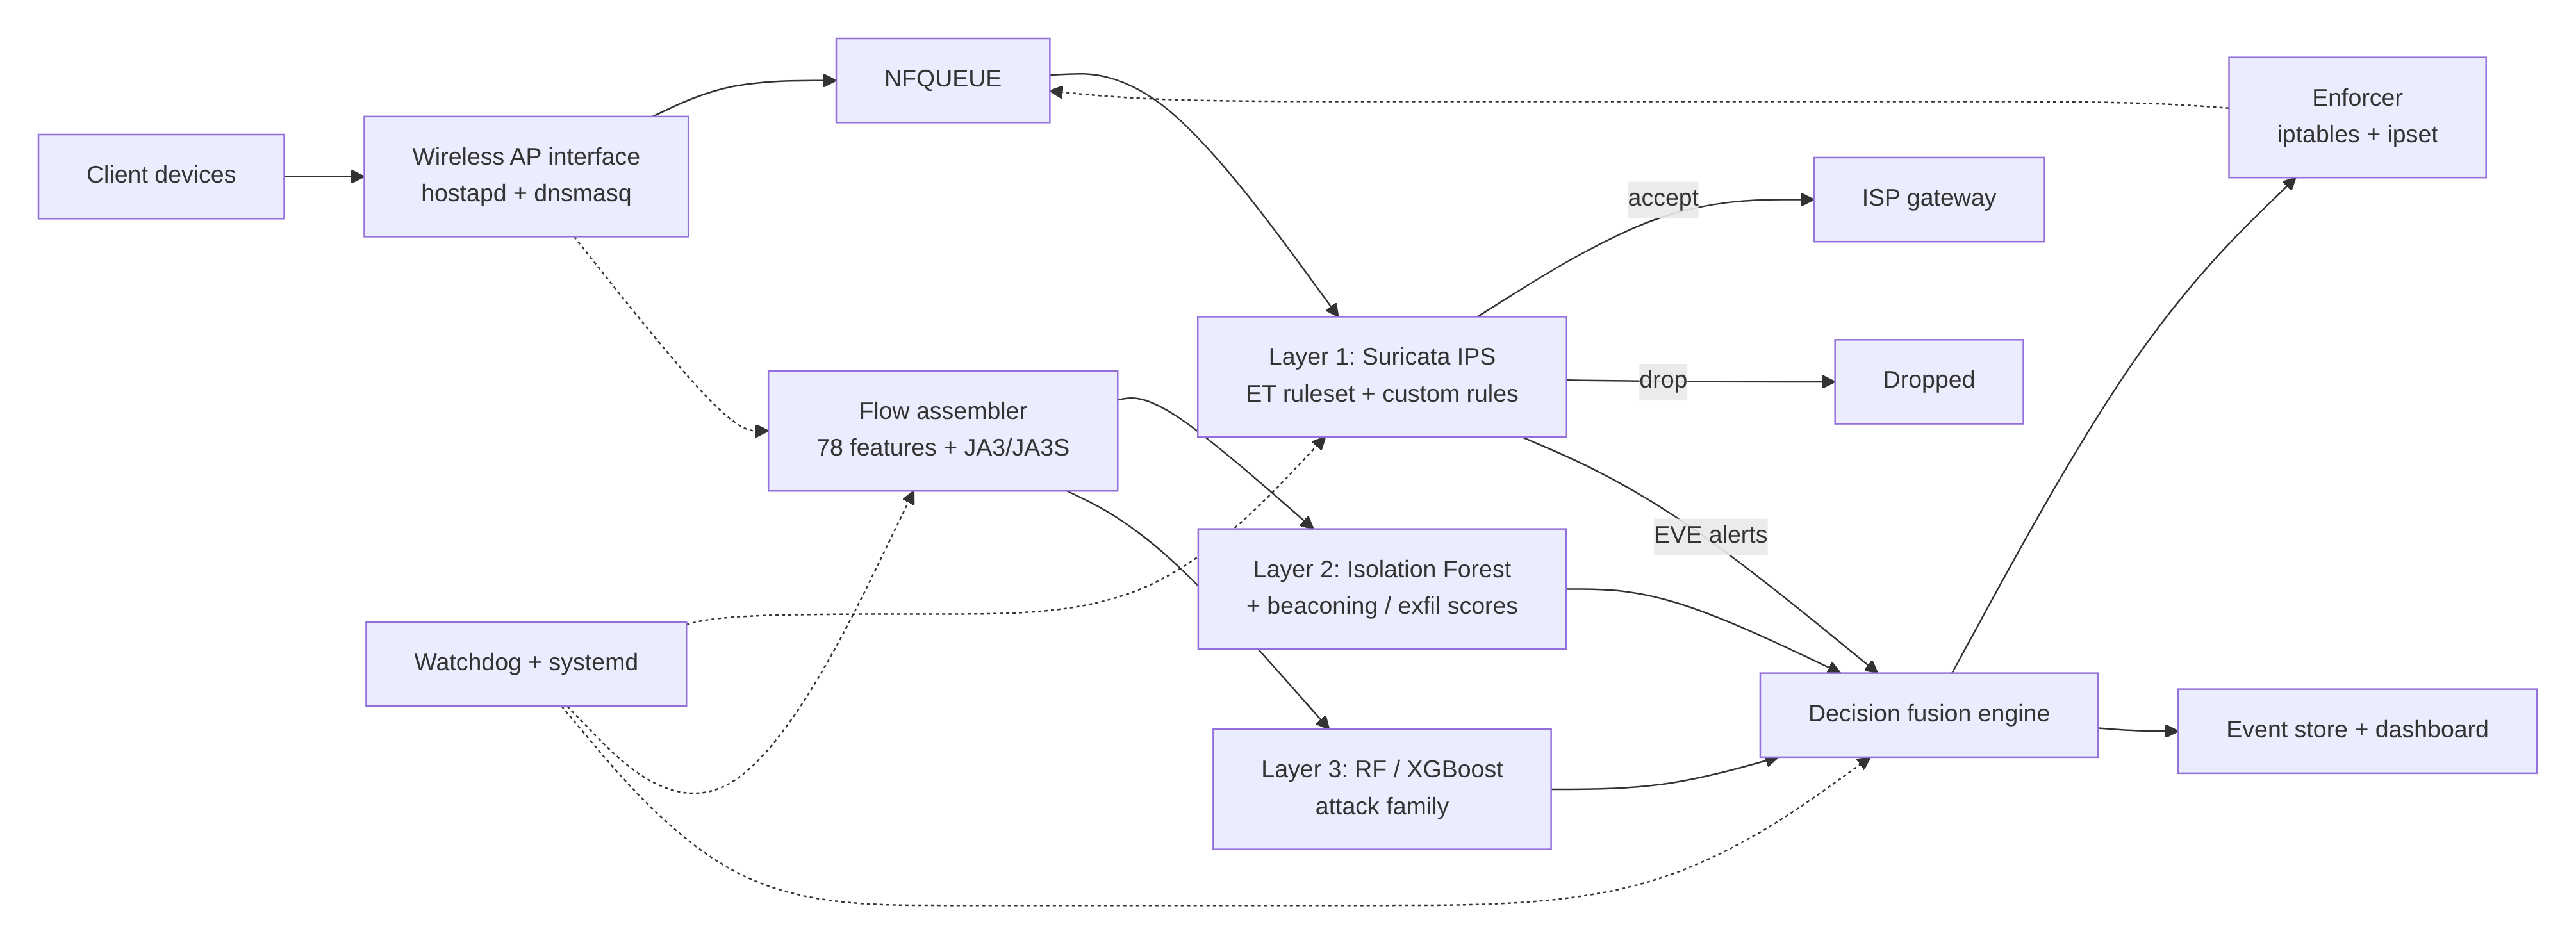
\includegraphics[width=\textwidth]{Figures/nidps_fig5_1.png}
    \caption{Proposed three-layer NIDPS pipeline.}
    \label{fig:pipeline}
\end{figure}

\noindent The design separates what must be fast from what can be thorough. Suricata decides per packet and adds only microseconds of forwarding delay. The machine learning layers decide per flow, so their verdicts are applied to the remainder of a long flow and to all later traffic from the offending host.

\section{Datasets}\label{sec:5.2}
\label{sec:datasets}
\noindent The machine learning layers are trained on three public intrusion detection benchmarks and evaluated additionally on traffic captured from our own deployment. The goal is not the highest score on one benchmark, but a model that still works when the training traffic and the deployment traffic differ.

\subsection{Public Benchmark Datasets}\label{sec:5.2.1}
\label{sec:public-datasets}
\noindent Table~\ref{tab:datasets} lists the public datasets used for training and cross-evaluation.

\begin{table}[H]
\centering
\caption{Public benchmark datasets used for training and cross-evaluation.}
\label{tab:datasets}
\begin{tabular}{|>{\raggedright\arraybackslash}p{0.17\linewidth}|>{\raggedright\arraybackslash}p{0.17\linewidth}|>{\raggedright\arraybackslash}p{0.22\linewidth}|>{\raggedright\arraybackslash}p{0.30\linewidth}|}
\hline
\textbf{Dataset} & \textbf{Source} & \textbf{Traffic profile} & \textbf{Attack families relevant to this project} \\
\hline
CIC-IDS-2017 \cite{nidps:cicids2017} & Canadian Institute for Cybersecurity (CIC) & 5 days of enterprise-style traffic & Brute force (SSH/FTP), DoS/DDoS, port scan, botnet, infiltration \\
\hline
CSE-CIC-IDS2018 \cite{nidps:cicids2018} & CIC with the Communications Security Establishment & Larger AWS-hosted network, 10 days & Brute force, DoS/DDoS, botnet, infiltration \\
\hline
CIC-IoT-2023 \cite{nidps:ciciot2023} & CIC & 105 IoT devices in a smart-home topology & DDoS, recon/scan, spoofing, brute force, Mirai-style attacks \\
\hline
\end{tabular}
\end{table}

\noindent CIC-IoT-2023 is closest to the target environment because home networks are increasingly dominated by IoT devices. CIC-IDS-2017 and CSE-CIC-IDS2018 contribute a wider range of host-based attacks. Published analyses of CIC-IDS-2017 have reported labelling and flow-construction errors in the original CSV files \cite{nidps:engelen2021}, which is one more reason flows are regenerated from the raw captures (Section~\ref{sec:harmonisation}).

\subsection{Self-Collected Real-World Dataset}\label{sec:5.2.2}
\label{sec:selfcollected}
\noindent A fourth dataset is captured on the deployed access point itself. It has two parts:
\begin{enumerate}
    \item \textbf{Benign capture.} Normal household or lab traffic (browsing, streaming, video calls, IoT devices, software updates) is recorded over several days. Flows that Suricata flags during this period are removed before the capture is labelled benign.
    \item \textbf{Attack capture.} Each in-scope attack is executed from a dedicated attacker machine in an isolated test network that we own, using standard penetration-testing tools. The start and end time, attacker address and target of each run are logged, so every flow in the window can be labelled automatically from these logs.
\end{enumerate}
\noindent This dataset is used only for testing, never for training. It measures how well models trained on public data transfer to a real home network.

\subsection{Feature Harmonisation Across Datasets}\label{sec:5.2.3}
\label{sec:harmonisation}
\noindent The public datasets do not share one feature format. The two CIC-IDS sets ship CICFlowMeter CSVs with about 80 columns whose names and rounding differ between releases, while CIC-IoT-2023 ships a different, smaller feature set computed over packet windows. A model trained on one format cannot be applied to another, and none of them is guaranteed to match what the live system computes.

\noindent To remove this mismatch, the following procedure is applied:
\begin{enumerate}
    \item Download the raw PCAP files of every dataset instead of the provided CSVs.
    \item Run the same flow extractor that runs on the device (Section~\ref{sec:flowassembly}) over every PCAP. All datasets then share an identical 78-feature schema, with identical definitions, timeouts and units. The extractor runs with the same timeouts as the device ($T_a = 10$\,s, $T_i = 30$\,s), so a training record and a live record always cover the same span of traffic.
    \item Re-label the regenerated flows by matching their 5-tuple and timestamps against each dataset's published attack schedule.
    \item Map every dataset-specific label onto one unified attack taxonomy (Table~\ref{tab:taxonomy}).
\end{enumerate}
\noindent The key advantage is that training-time and serving-time features are produced by the same code, so there is no train/serve skew.

\begin{table}[H]
\centering
\caption{Unified attack taxonomy used for Layer 3.}
\label{tab:taxonomy}
\begin{tabular}{|>{\raggedright\arraybackslash}p{0.24\linewidth}|>{\raggedright\arraybackslash}p{0.46\linewidth}|>{\raggedright\arraybackslash}p{0.16\linewidth}|}
\hline
\textbf{Unified class} & \textbf{Examples of original labels} & \textbf{Primary detecting layer} \\
\hline
Benign & BENIGN, BenignTraffic & -- \\
\hline
Reconnaissance & PortScan, Recon-PortScan, Recon-OSScan & L1, L3 \\
\hline
Brute force & SSH-Patator, FTP-Patator, DictionaryBruteForce & L1, L3 \\
\hline
DoS / DDoS & DoS Hulk, DDoS LOIC, DDoS-SYN\_Flood, DDoS-UDP\_Flood & L1, L3 \\
\hline
Botnet / C2 & Bot, Mirai variants & L2, L3 \\
\hline
Spoofing & DNS\_Spoofing, MITM-ArpSpoofing & L1 \\
\hline
Infiltration / lateral movement & Infiltration, internal scanning after compromise & L3 \\
\hline
\end{tabular}
\end{table}

\subsection{Pre-processing}\label{sec:5.2.4}
\label{sec:preprocessing}
\noindent The regenerated flow tables are cleaned before training:
\begin{itemize}
    \item \textbf{Invalid values:} rows with infinite or undefined values (for example, rates computed over a zero-length flow) are dropped, and exact duplicate rows are removed.
    \item \textbf{Identifier removal:} source and destination IP addresses, ports, flow IDs and timestamps are removed from the feature vector. They identify the lab, not the attack, and keeping them lets a model memorise the attacker's address instead of learning behaviour.
    \item \textbf{Constant features:} features with zero variance in the training set are removed.
    \item \textbf{Splitting:} within one dataset, the split into training and test sets is done by capture day rather than at random, because neighbouring flows of the same attack run are nearly identical and a random split leaks them into both sets.
    \item \textbf{Class imbalance:} class proportions are heavily skewed, in opposite directions: benign flows dominate CIC-IDS-2017, while attack flows dominate CIC-IoT-2023. Layer 3 uses class weights inversely proportional to class frequency; oversampling (SMOTE), if used, is applied only to the training fold.
    \item \textbf{Scaling:} tree-based models do not need feature scaling, so values are kept in their original units. This also keeps the online pipeline simple.
    \item \textbf{Isolation Forest training set:} Layer 2 is trained only on benign flows, since it models normal behaviour.
\end{itemize}

\section{Traffic Acquisition and Flow Construction}\label{sec:5.3}
\label{sec:acquisition}
\noindent All detection depends on how packets reach the detectors and how they are summarised. This section describes the inline packet path, the flow assembly algorithm and the extraction of TLS fingerprints from encrypted traffic.

\subsection{Inline Packet Path}\label{sec:5.3.1}
\label{sec:packetpath}
\noindent The host runs hostapd to expose a wireless network and dnsmasq to provide DHCP and DNS to clients. IP forwarding is enabled and the uplink interface performs NAT towards the ISP gateway. Forwarded traffic is diverted by an iptables rule in the FORWARD chain to an NFQUEUE, where Suricata runs in IPS mode. For each packet, Suricata returns an accept or drop verdict to the kernel.

\noindent A copy of every forwarded packet is also read by the flow assembler through a packet capture socket on the wireless interface. The flow assembler never holds packets back, so a slow ML layer cannot slow down forwarding.

\noindent One platform detail matters for lateral movement. By default, the wireless driver and hostapd relay frames between two wireless clients directly, without passing them up to the IP layer, so netfilter and Suricata never see them. To inspect client-to-client traffic, client isolation (\texttt{ap\_isolate=1}) is enabled and intra-network traffic is routed through the host. Without this setting, lateral movement can only be detected when it crosses the AP's IP layer.

\subsection{Flow Assembly Algorithm}\label{sec:5.3.2}
\label{sec:flowassembly}
\noindent A flow is the set of packets sharing the same 5-tuple (source IP, destination IP, source port, destination port, protocol) in either direction. The direction of the first packet defines ``forward''; replies are ``backward''. Algorithm~\ref{alg:flow} shows how flows are built and closed.

\begin{algorithm}[H]
\caption{Bidirectional flow assembly}
\label{alg:flow}
\KwIn{packet stream $P$; active timeout $T_a$ (default 10\,s); idle timeout $T_i$ (default 30\,s)}
\KwOut{completed flow records with 78 features}
$FlowTable \leftarrow$ empty hash map keyed by canonical 5-tuple\;
\ForEach{packet $p \in P$}{
    $k \leftarrow \mathrm{canonical}(p.\mathrm{5tuple})$ \tcp*{same key for both directions}
    \If{$k \notin FlowTable$}{
        create flow $f$ with $f.start \leftarrow p.time$ and $f.fwd \leftarrow$ direction of $p$\;
        $FlowTable[k] \leftarrow f$\;
    }
    $f \leftarrow FlowTable[k]$\;
    update the running statistics of $f$ with $p$ (direction, size, flags, time)\;
    \If{$p$ carries a TLS ClientHello or ServerHello}{
        attach JA3/JA3S to $f$ (Algorithm~\ref{alg:ja3})\;
    }
    \uIf{$p$ has FIN in both directions or RST}{
        emit($f$)\; remove $k$\;
    }
    \ElseIf{$p.time - f.start \geq T_a$}{
        emit($f$) as a partial record\; reset the counters of $f$ but keep $k$\;
    }
}
\tcp{run periodically}
\ForEach{flow $f$ with $now - f.last\_seen \geq T_i$}{
    emit($f$)\; remove its key\;
}
\end{algorithm}

\noindent The active timeout lets a long-running connection, such as a slow exfiltration channel, be scored in segments while it is still open, instead of only when it closes. Each segment is emitted as its own flow record, after which its counters reset. The idle timeout reclaims memory from flows that stop without a FIN or RST. Table~\ref{tab:timeouts} gives the default values.

\begin{table}[H]
\centering
\caption{Flow timeout parameters.}
\label{tab:timeouts}
\begin{tabular}{|>{\raggedright\arraybackslash}p{0.22\linewidth}|>{\raggedright\arraybackslash}p{0.24\linewidth}|>{\raggedright\arraybackslash}p{0.42\linewidth}|}
\hline
\textbf{Parameter} & \textbf{Default} & \textbf{Effect} \\
\hline
Active timeout $T_a$ & 10\,s (configurable, e.g.\ 5--30\,s) & An open flow is re-scored every $T_a$, which caps how long one connection can run unscored \\
\hline
Idle timeout $T_i$ & 30\,s & A flow with no packets for $T_i$ is closed and scored \\
\hline
\end{tabular}
\end{table}

\noindent Most flows, such as web requests, DNS lookups and scan probes, end in well under 5 seconds and are scored once, when they close. Only long-lived connections are segmented. $T_a$ trades CPU for reaction time: halving it doubles the scoring work for long flows. The default of 10\,s is a conservative starting point for low-cost hardware. $T_a$ is a configuration parameter, so a deployment with spare CPU can lower it, for example to 5\,s, to react faster. The evaluation measures both settings (Section~\ref{sec:sysperf}).

\noindent The 78 features follow the CICFlowMeter definitions: packet and byte counts per direction, packet length statistics, inter-arrival time statistics, TCP flag counts, header lengths, bulk and sub-flow measures, and active/idle periods. To keep memory constant per flow, means and variances are updated incrementally with Welford's method (Equation~\ref{eq:welford}) rather than by storing every packet:
\begin{equation}
\label{eq:welford}
\begin{aligned}
\mu_n &= \mu_{n-1} + \frac{x_n - \mu_{n-1}}{n}, \\
M_n &= M_{n-1} + (x_n - \mu_{n-1})(x_n - \mu_n), \\
\sigma_n^2 &= \frac{M_n}{n-1}.
\end{aligned}
\end{equation}
\noindent Here $x_n$ is the $n$-th observation (for example, a packet length), $\mu_n$ the running mean and $M_n$ the running sum of squared deviations. Minimum and maximum are tracked directly.

\subsection{TLS Fingerprint Extraction (JA3/JA3S)}\label{sec:5.3.3}
\label{sec:ja3}
\noindent Most traffic is encrypted, so payload cannot be inspected without decryption. Decrypting traffic on the AP would require installing a certificate on every client, would break certificate pinning in many apps and would cost far more CPU than the target hardware can spare. Instead, the system uses fields of the TLS handshake that are sent in clear text \cite{nidps:ja3}, as shown in Algorithm~\ref{alg:ja3}.

\begin{algorithm}[H]
\caption{JA3/JA3S fingerprint}
\label{alg:ja3}
\KwIn{TLS ClientHello (or ServerHello)}
\KwOut{32-character MD5 fingerprint}
read the TLS version, cipher suites, extension types, supported groups (elliptic curves) and EC point formats\;
remove GREASE values (0x0a0a, 0x1a1a, \ldots, 0xfafa) from every list\;
join the decimal values of each list with ``-''\;
$s_{JA3} \leftarrow$ Version,Ciphers,Extensions,Groups,PointFormats\;
$s_{JA3S} \leftarrow$ Version,Cipher,Extensions \tcp*{ServerHello}
\Return{MD5($s$)}\;
\end{algorithm}

\noindent The fingerprint identifies the client software that opened the connection, not the user. Malware and C2 frameworks often use TLS libraries with fingerprints that differ from common browsers and operating systems. The pair (JA3, JA3S) is attached to the flow record and used by Layer 2 in two ways: as a rarity signal (how many local hosts have ever used this fingerprint) and as part of the key for beacon detection (Section~\ref{sec:beacon}). Suricata's TLS parser can emit the same hashes in its EVE logs, which lets Layer 1 rules match known-bad fingerprints directly.

\section{Layer 1: Signature-Based Detection}\label{sec:5.4}
\label{sec:layer1}
\noindent Layer 1 catches attacks that have a known, stable pattern. It is the only layer that acts on individual packets, so it is the first line of prevention.

\subsection{Suricata Configuration}\label{sec:5.4.1}
\label{sec:suricata}
\noindent Suricata \cite{nidps:suricata} runs in IPS mode on the NFQUEUE with the Emerging Threats Open ruleset. Rule categories that do not apply to a home network (for example, SCADA protocols) are disabled to save CPU. Each rule carries an action (alert or drop) and a severity from 1 (highest) to 3. Rules with severity 1 that target in-scope attacks are set to drop; the rest only alert and are passed on to decision fusion. Every alert is written to Suricata's EVE JSON output, which the alert ingestor reads over a Unix socket.

\subsection{Custom Rules for In-Scope Attacks}\label{sec:5.4.2}
\label{sec:customrules}
\noindent The ET ruleset matches known payloads well, but several in-scope attacks are defined by rate rather than content. These are covered by custom threshold rules, which count matching events per source address within a time window (Table~\ref{tab:customrules}).

\begin{table}[H]
\centering
\caption{Custom Layer 1 rules for the in-scope attacks.}
\label{tab:customrules}
\begin{tabular}{|>{\raggedright\arraybackslash}p{0.2\linewidth}|>{\raggedright\arraybackslash}p{0.42\linewidth}|>{\raggedright\arraybackslash}p{0.24\linewidth}|}
\hline
\textbf{Attack} & \textbf{Detection logic} & \textbf{Example threshold (tunable)} \\
\hline
SSH brute force & New TCP connections (SYN) to port 22 from one source & $\geq 5$ in 60\,s \\
\hline
Port scan & SYN packets from one source to many distinct destination ports & $\geq 20$ ports in 10\,s \\
\hline
DNS spoofing & DNS responses to clients whose source is not the AP's own resolver & any occurrence \\
\hline
Known C2 TLS client & JA3 hash on a blocklist of published malicious fingerprints & any occurrence \\
\hline
SYN flood (DoS) & SYN packets to one destination without completed handshakes & rate above a calibrated limit \\
\hline
\end{tabular}
\end{table}

\noindent The thresholds are starting values that are tuned during evaluation. The DNS spoofing rule relies on the AP design. Clients receive the AP's address as their only DNS server through DHCP, so a legitimate DNS answer always comes from the AP. Any DNS response arriving at a client from another address is forged or comes from a rogue resolver.

\subsection{ARP Spoofing Monitor}\label{sec:5.4.3}
\label{sec:arp}
\noindent Suricata inspects IP traffic and does not match rules against ARP frames, which sit below the IP layer. ARP spoofing is therefore detected by a small companion sensor that belongs to Layer 1 and reports into the same alert stream. It uses the DHCP lease table of dnsmasq as the ground truth for which MAC address owns which IP address (Algorithm~\ref{alg:arp}).

\begin{algorithm}[H]
\caption{ARP consistency check}
\label{alg:arp}
\KwIn{ARP frames on the wireless interface; DHCP lease table $L$ (IP $\rightarrow$ MAC)}
\KwOut{ARP spoofing alerts}
$Bindings \leftarrow L$ \tcp*{trusted IP-to-MAC map}
\ForEach{ARP reply or gratuitous ARP $a$}{
    \If{$a.sender\_ip \in Bindings$ \textbf{and} $Bindings[a.sender\_ip] \neq a.sender\_mac$}{
        raise alert ARP\_SPOOF (attacker $a.sender\_mac$, victim $a.sender\_ip$)\;
    }
    \If{$a.sender\_ip = gateway\_ip$ \textbf{and} $a.sender\_mac \neq AP\_mac$}{
        raise alert GATEWAY\_IMPERSONATION with severity 1\;
    }
    \If{more than $N$ unsolicited replies from one MAC within window $W$}{
        raise alert ARP\_FLOOD\;
    }
}
on every DHCP lease change, refresh $Bindings$ from $L$\;
\end{algorithm}

\noindent Impersonating the gateway is the classic step before a man-in-the-middle attack, so that check raises the highest severity.

\section{Layer 2: Unsupervised Anomaly Detection}\label{sec:5.5}
\label{sec:layer2}
\noindent Layer 2 flags traffic that looks unlike the network's normal behaviour, without needing a label for the attack. It covers what signatures miss: new attacks, variants that change their signature, C2 beaconing and data exfiltration.

\subsection{Isolation Forest}\label{sec:5.5.1}
\label{sec:iforest}
\noindent Isolation Forest \cite{nidps:iforest} is based on a simple observation: anomalies are few and different, so they are easier to separate from the rest of the data than normal points are. The model builds an ensemble of random binary trees. Each tree is grown on a random subsample of $\psi$ flows by repeatedly choosing a random feature and a random split value between that feature's minimum and maximum, until every point is isolated or a height limit of $\lceil \log_2 \psi \rceil$ is reached.

\noindent An anomalous flow is isolated after few splits, so its path length $h(x)$ from root to leaf is short. Averaging over all trees gives $E[h(x)]$, which is normalised by the average path length of an unsuccessful search in a binary search tree of $\psi$ points:
\begin{equation}
\label{eq:cpsi}
c(\psi) = 2H(\psi - 1) - \frac{2(\psi - 1)}{\psi}, \qquad H(i) \approx \ln(i) + 0.5772
\end{equation}
\begin{equation}
\label{eq:ifscore}
s(x, \psi) = 2^{-\frac{E[h(x)]}{c(\psi)}}
\end{equation}
\noindent The anomaly score $s$ in Equation~\ref{eq:ifscore} lies between 0 and 1. Scores close to 1 indicate clear anomalies; scores well below 0.5 indicate normal points. The model uses $t = 100$ trees and $\psi = 256$, the values recommended by the original authors, and is trained only on benign flows from the harmonised datasets.

\noindent Isolation Forest suits the target hardware because training and scoring are cheap. Scoring a flow costs $t$ tree walks of at most $\lceil \log_2 \psi \rceil = 8$ steps each, regardless of how much training data was used.

\subsection{Adaptive Threshold Calibration}\label{sec:5.5.2}
\label{sec:calibration}
\noindent The model outputs a continuous score, so a threshold $\tau$ is needed to turn it into a decision. A threshold taken from benchmark traffic does not fit every home network: a household with game consoles and security cameras produces traffic that a benchmark lab never saw, which shows up as false positives. The calibration scheme in Algorithm~\ref{alg:calibration} adjusts only the threshold to each deployment; it does not retrain the model.

\begin{algorithm}[H]
\caption{Per-network threshold calibration}
\label{alg:calibration}
\KwIn{trained Isolation Forest $M$; global threshold $\tau_g$; calibration window $W$ (e.g.\ 24--72\,h); percentile $p$ (e.g.\ 99.5); minimum sample count $N_{min}$; maximum shift $\delta$}
\KwOut{calibration state $\{\tau, \mathrm{timestamp}, n\}$}
$S \leftarrow \emptyset$\;
\ForEach{flow $x$ completed during $W$}{
    \If{$x$ matched any Suricata alert \textbf{or} came from a blocked host}{
        skip $x$ \tcp*{keep the baseline clean}
    }
    add $M.\mathrm{score}(x)$ to $S$\;
}
\eIf{$|S| < N_{min}$}{
    $\tau \leftarrow \tau_g$ \tcp*{too little local data: fall back}
}{
    $\tau_l \leftarrow p$-th percentile of $S$\;
    $\tau \leftarrow \mathrm{clip}(\tau_l,\ \tau_g - \delta,\ \tau_g + \delta)$\;
}
store $\{\tau, now, |S|\}$ as calibration metadata\;
repeat periodically (e.g.\ weekly) as the network's traffic changes\;
\end{algorithm}

\noindent Two safeguards protect the calibration. The exclusion step leaves out flows that Layer 1 already considers malicious. The clipping step limits how far the local threshold may move from the global one, so an attacker who is active during calibration cannot raise the threshold far enough to hide.

\noindent The percentile $p$ directly sets the expected false positive rate on the calibration traffic: with $p = 99.5$, about 0.5\% of benign local flows would exceed $\tau$. This makes the trade-off between missed attacks and alert volume an explicit, tunable parameter.

\subsection{Data Exfiltration Score}\label{sec:5.5.3}
\label{sec:exfil}
\noindent Exfiltration is a property of a host over time, not of one flow. For each internal host $h$, the system keeps an exponentially weighted moving average and variance of its outbound bytes per time bucket $b_t$ (60\,s by default):
\begin{equation}
\label{eq:ewma}
\bar{b}_t = \alpha\, b_t + (1 - \alpha)\, \bar{b}_{t-1}, \qquad
\sigma_t^2 = \alpha\, (b_t - \bar{b}_{t-1})^2 + (1 - \alpha)\, \sigma_{t-1}^2
\end{equation}
\noindent A bucket is flagged when $b_t$ exceeds the host's baseline by $k$ standard deviations ($k = 4$ as a starting value) and the outbound-to-inbound byte ratio of the host's flows is also unusually high. The second condition prevents large uploads that are part of normal two-way activity, such as video calls, from triggering the alert.

\noindent Bucket statistics react only once per bucket, so a second, faster check runs on every active-timeout segment. If one segment carries more than $U_{max}$ bytes outbound to a destination the host has never contacted before, a high-weight evidence item is raised immediately. $U_{max}$ is set during calibration (Algorithm~\ref{alg:calibration}) as a high percentile, for example the 99.9th, of segment upload sizes in local benign traffic. When this evidence leads to a block, leakage over a single connection is bounded by roughly the host's upload rate $\times$ ($T_a$ + scoring delay). At 20\,Mbps and the default $T_a = 10$\,s, that is about 25\,MB.

\subsection{C2 Beaconing Score}\label{sec:5.5.4}
\label{sec:beacon}
\noindent Infected devices typically contact their command-and-control server at regular intervals. Flows are grouped by the key (internal host, destination IP or TLS server name, JA3). For each group with at least $m$ connections in the observation window, the inter-arrival times $\Delta t_1, \ldots, \Delta t_k$ between consecutive connections are computed, along with their coefficient of variation:
\begin{equation}
\label{eq:cv}
CV = \frac{\sigma_{\Delta t}}{\mu_{\Delta t}}
\end{equation}
\noindent Human-driven traffic is irregular (high $CV$), while beacons are close to periodic (low $CV$), even with added random jitter. The beacon score combines three signals: a low $CV$, a low variance in bytes per connection, and a rare JA3 fingerprint on the local network. A group is reported when all three point the same way, which keeps legitimate periodic traffic, such as software update checks from common browsers, from being flagged.

\section{Layer 3: Supervised Attack Classification}\label{sec:5.6}
\label{sec:layer3}
\noindent Layer 3 assigns each flow to one of the unified classes of Table~\ref{tab:taxonomy}. Where Layer 2 answers ``is this unusual?'', Layer 3 answers ``which known kind of attack does this look like?''. The class label decides the response and makes alerts readable on the dashboard. Two tree ensembles are trained and compared, and the better one under the hardware budget is deployed.

\subsection{Random Forest}\label{sec:5.6.1}
\label{sec:rf}
\noindent Random Forest \cite{nidps:rf} trains many decision trees, each on a bootstrap sample of the training flows, and at each split considers only a random subset of $\sqrt{d}$ of the $d$ features. Splits are chosen to minimise Gini impurity:
\begin{equation}
\label{eq:gini}
G(S) = 1 - \sum_{k=1}^{K} p_k^2
\end{equation}
\noindent where $p_k$ is the share of class $k$ among the flows $S$ at a node. The forest predicts by averaging the class probabilities of all trees. Bootstrapping and feature subsampling make the trees disagree in useful ways, so the ensemble is less prone to overfitting than a single tree. This matters because the model is trained on lab traffic and deployed on a different network.

\subsection{XGBoost}\label{sec:5.6.2}
\label{sec:xgb}
\noindent XGBoost \cite{nidps:xgb} builds trees one after another, each new tree correcting the errors of the current ensemble. It minimises a regularised objective:
\begin{equation}
\label{eq:xgb}
\mathcal{L} = \sum_{i} l(y_i, \hat{y}_i) + \sum_{m} \Omega(f_m), \qquad
\Omega(f) = \gamma T + \tfrac{1}{2} \lambda \lVert w \rVert^2
\end{equation}
\noindent Here $l$ is the multi-class log loss, $T$ is the number of leaves of tree $f$ and $w$ its leaf weights. The $\gamma$ and $\lambda$ terms penalise large, complex trees. XGBoost is usually more accurate than Random Forest on tabular data, but it is more sensitive to hyperparameters and can fit dataset-specific artefacts more closely, which the cross-dataset evaluation (Section~\ref{sec:crossdataset}) is designed to expose.

\subsection{Training and Model Selection}\label{sec:5.6.3}
\label{sec:modelselection}
\begin{enumerate}
    \item Train on the harmonised flows with identifiers removed (Section~\ref{sec:preprocessing}), using class weights to counter imbalance.
    \item Tune hyperparameters (number of trees, maximum depth, learning rate for XGBoost, minimum samples per leaf) with stratified 5-fold cross-validation on the training days only.
    \item Select by macro-averaged F1-score rather than accuracy. With heavily skewed classes, a model that always predicts the majority class can still look accurate while missing the rare classes entirely.
    \item Apply a hardware budget: among models within one F1 point of the best, choose the one with the lowest per-flow inference time and memory on the target device.
    \item Export the chosen model with its feature list and version number, so the runtime refuses a model whose features do not match the extractor.
\end{enumerate}

\subsection{Confidence Handling}\label{sec:5.6.4}
\label{sec:confidence}
\noindent The classifier always outputs a probability vector $p$ over the $K$ classes. The predicted class is $\hat{y} = \arg\max p$, with confidence $c = \max p$. Low confidence means the flow does not fit any class well, which often happens with attacks the model never saw. Instead of forcing a label, flows with $c$ below a confidence threshold $\theta_c$ are labelled ``unknown'' and passed to decision fusion with their Layer 2 score. This way, Layer 3 refines detections but does not overrule a strong anomaly signal.

\section{Decision Fusion}\label{sec:5.7}
\label{sec:fusion}
\noindent The three layers can disagree, and acting on any single one would either block too much (anomaly scores alone are noisy) or too little (signatures alone miss new attacks). The decision-fusion engine combines their evidence per flow and per host. Its main principle is that strong evidence from one layer is enough to block, while weak evidence must be confirmed by a second layer or must accumulate over time.

\subsection{Verdict Algorithm}\label{sec:5.7.1}
\label{sec:verdict}
\noindent Algorithm~\ref{alg:verdict} gives the per-flow verdict, and Figure~\ref{fig:fusion} shows the same logic as a flowchart.

\begin{algorithm}[H]
\caption{Per-flow verdict}
\label{alg:verdict}
\KwIn{flow $f$; Suricata alerts $A(f)$; anomaly score $s(f)$; threshold $\tau$; class probabilities $p(f)$; thresholds $\theta_{block} > \theta_{alert} > \theta_c$}
\KwOut{verdict in \{PASS, ALERT, BLOCK\} and the attributed layer(s)}
\lIf{$f.src \in$ allowlist}{\Return{PASS}}
\lIf{$A(f)$ contains a drop rule or severity 1}{\Return{BLOCK, layer L1}}
$y \leftarrow \arg\max p(f)$; \quad $c \leftarrow \max p(f)$\;
\lIf{$y \neq$ Benign \textbf{and} $c \geq \theta_{block}$}{\Return{BLOCK, layer L3}}
\lIf{$s(f) \geq \tau$ \textbf{and} $y \neq$ Benign \textbf{and} $c \geq \theta_{alert}$}{\Return{BLOCK, layers L2+L3}}
\If{$s(f) \geq \tau$ \textbf{or} $A(f) \neq \emptyset$ \textbf{or} ($y \neq$ Benign \textbf{and} $c \geq \theta_{alert}$)}{
    add evidence to the host score of $f.src$ (Section~\ref{sec:hostscore})\;
    \Return{ALERT}\;
}
\Return{PASS}\;
\end{algorithm}

\noindent A confident known attack is blocked on Layer 3 alone, while a less confident classification is blocked only when Layer 2 agrees.

\begin{figure}[!htbp]
    \centering
    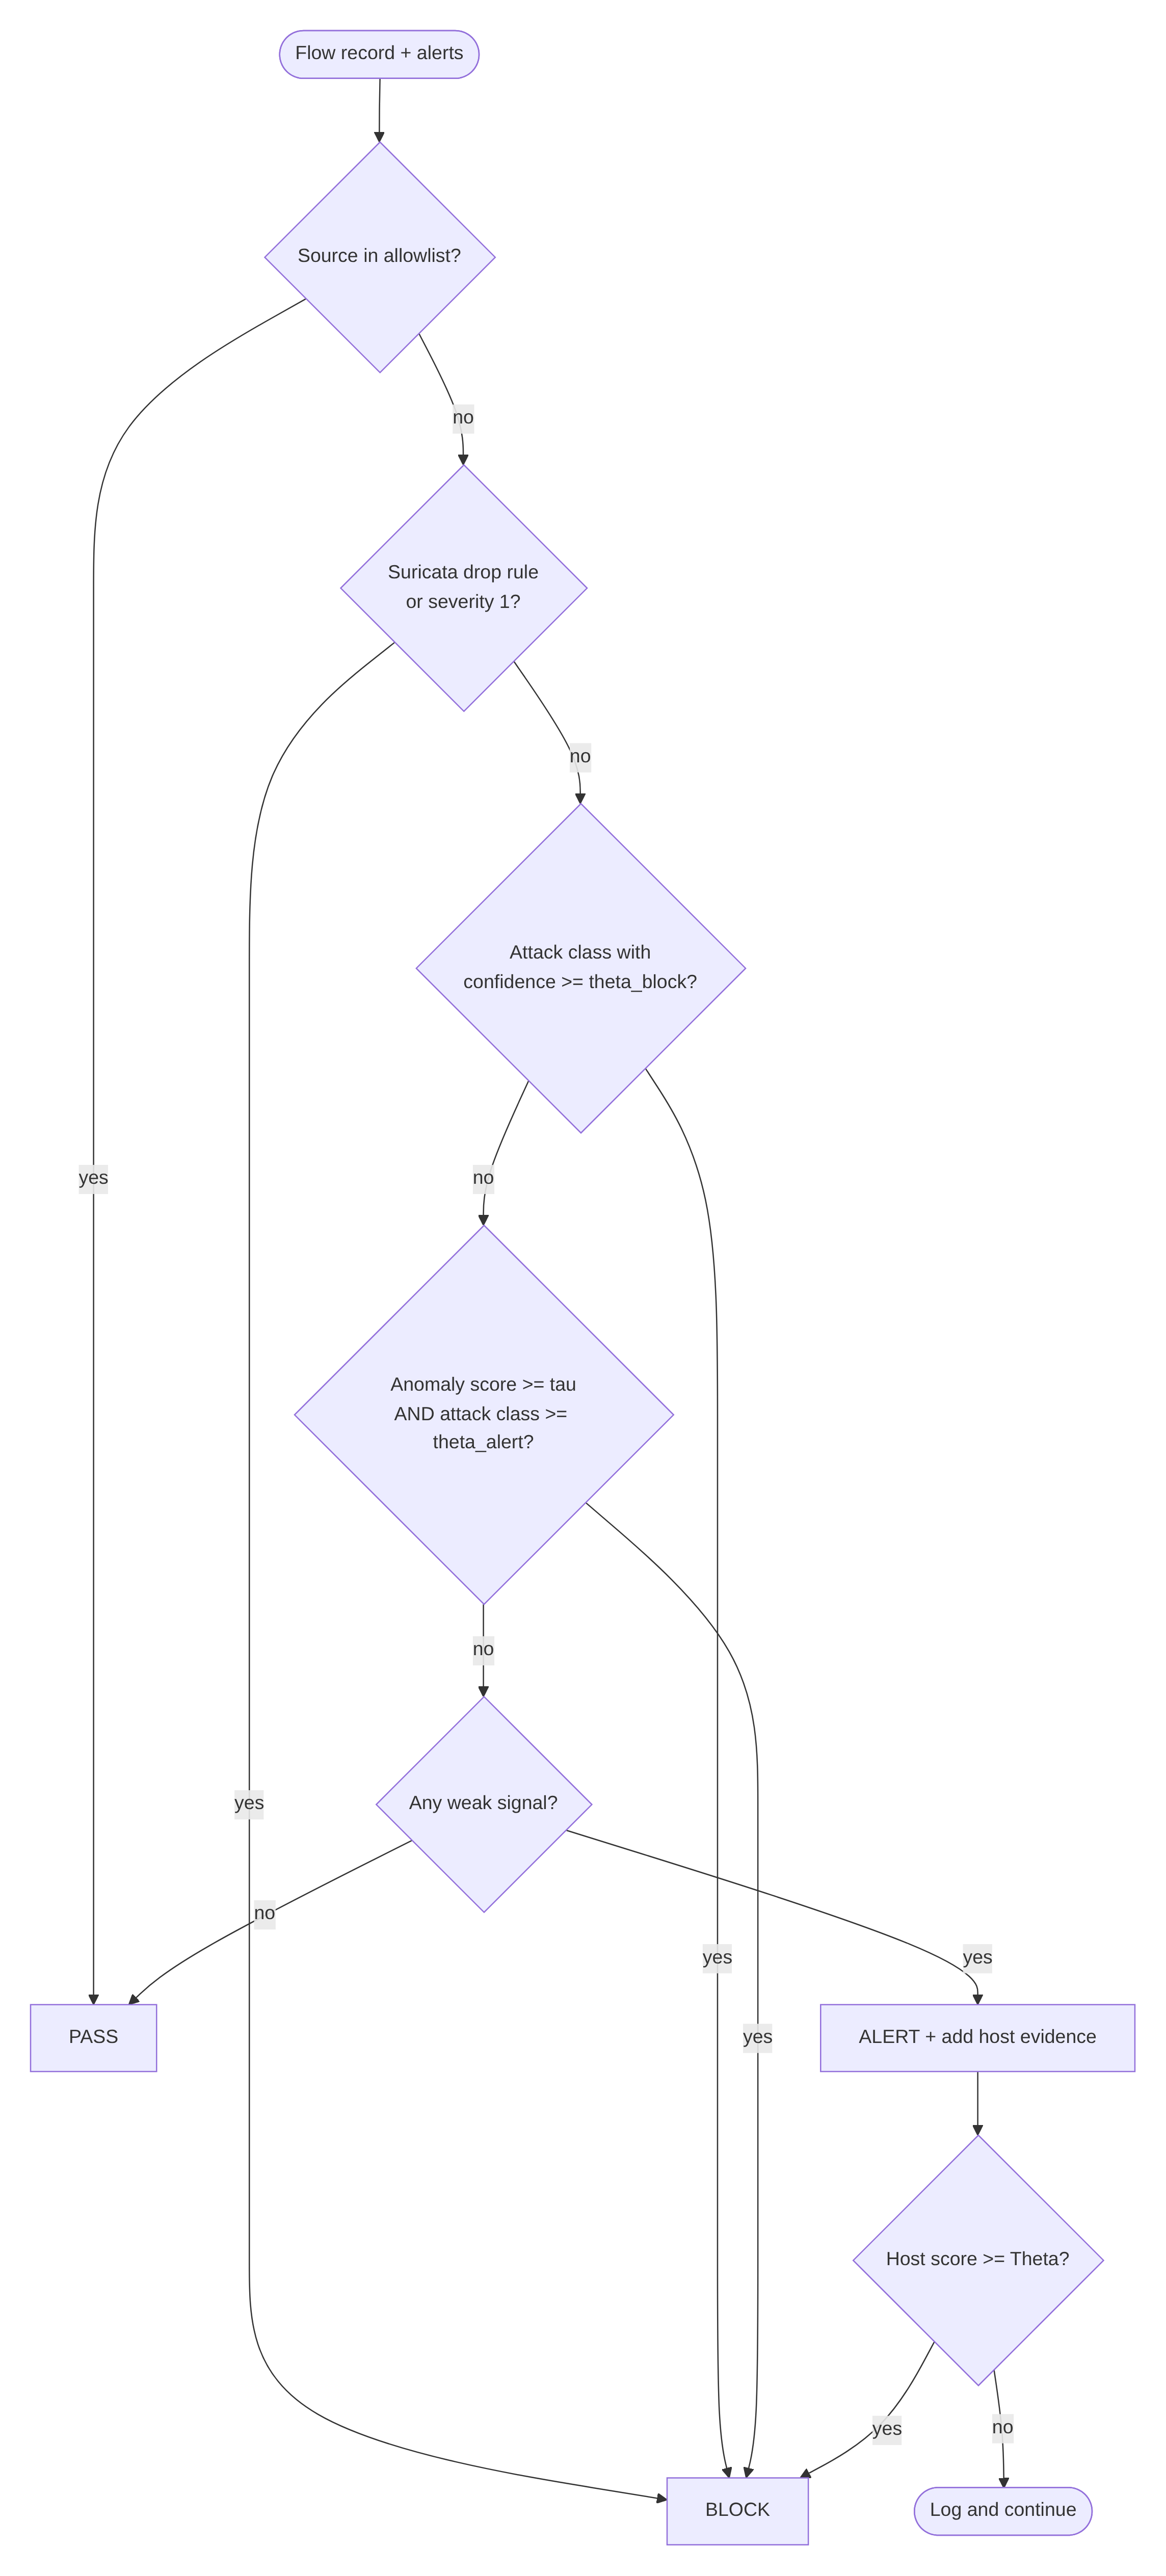
\includegraphics[width=0.62\textwidth]{Figures/nidps_fig5_2.png}
    \caption{Decision-fusion flow for one flow record.}
    \label{fig:fusion}
\end{figure}

\subsection{Host Evidence Accumulation}\label{sec:5.7.2}
\label{sec:hostscore}
\noindent Some attacks, such as a slow port scan or low-volume exfiltration, never produce one strong signal. Their individual flows only trigger alerts. The host score $S_h$ collects this weak evidence and lets it fade over time, so that a single stray alert does not lead to a block but a steady stream of alerts does:
\begin{equation}
\label{eq:hostscore}
S_h(t) = S_h(t_{prev})\, e^{-\lambda (t - t_{prev})} + w_v
\end{equation}
\noindent Here $w_v$ is the weight of the new alert (for example, higher for a Suricata alert than for an anomaly score just above $\tau$) and $\lambda$ is a decay rate. With a half-life of 10 minutes, $\lambda = \ln 2 / 600\ \mathrm{s}^{-1}$. When $S_h$ reaches the block threshold $\Theta$, the host is blocked. The same score is shown on the dashboard as the host's current risk level.

\subsection{Timing of ML Verdicts}\label{sec:5.7.3}
\label{sec:mltiming}
\noindent Layers 2 and 3 score completed flows or active-timeout segments (Algorithm~\ref{alg:flow}), so their verdict comes after part of the traffic has passed. Their blocks therefore apply to the rest of a long flow and to all later traffic from that source. This is acceptable for the attacks they target: beaconing, exfiltration, DDoS and lateral movement all unfold over many flows. Attacks that must be stopped at the first packet are the responsibility of Layer 1.

\noindent With the default $T_a = 10$\,s, the worst-case delay for an ML verdict on a long flow is about 10 seconds plus scoring time, which is milliseconds for tree models. The data that can leave over one connection before a block is therefore roughly the upload rate $\times$ that delay. This exposure is measured directly in the live exfiltration tests as ``bytes leaked before block'' (Table~\ref{tab:sysperf}), rather than estimated.

\section{Automated Prevention}\label{sec:5.8}
\label{sec:prevention}
\noindent A BLOCK verdict is turned into a firewall entry by the enforcer. The enforcer must stop attacks quickly without ever locking the owner out of their own network, so blocking follows a strict procedure.

\subsection{Blocking Mechanism}\label{sec:5.8.1}
\label{sec:blockmech}
\noindent Blocked addresses are stored in an ipset with a per-entry timeout, referenced by a single iptables rule placed before the NFQUEUE rule in the FORWARD chain (and in INPUT, to protect the AP itself). Adding or removing an address changes only the set, not the rule list, so a block takes effect immediately and costs the same regardless of how many addresses are blocked. Entries expire automatically, so a block never outlives its intended duration even if the enforcer crashes.

\subsection{Blocking Procedure}\label{sec:5.8.2}
\label{sec:blockproc}
\noindent Algorithm~\ref{alg:block} gives the procedure followed for every BLOCK verdict.

\begin{algorithm}[H]
\caption{Enforce a BLOCK verdict}
\label{alg:block}
\KwIn{offending address $a$; attack class $y$; attributed layer(s)}
\KwOut{ipset entry and audit record}
\If{$a \in$ allowlist (AP, gateway, DNS resolver, admin devices)}{
    log ``block suppressed''\; \Return{}\;
}
\If{blocks issued in the last minute $\geq R_{max}$}{
    downgrade to ALERT\; raise a ``block rate limit'' warning\; \Return{}\;
}
$n \leftarrow$ number of earlier blocks of $a$ within 24\,h\;
$duration \leftarrow \min(D_0 \cdot 2^n,\ D_{max})$ \tcp*{e.g.\ $D_0 = 5$\,min, $D_{max} = 24$\,h}
add $a$ to the ipset with timeout $duration$\;
write audit record $\{a, y, \mathrm{layers}, duration, \mathrm{evidence}, \mathrm{time}\}$\;
push the event to the dashboard\;
\end{algorithm}

\noindent The allowlist check prevents the system from cutting off its own infrastructure, even when an attacker forges packets from those addresses. The rate limit stops a flood of false positives, or an attacker spoofing many sources, from turning the NIDPS into a denial-of-service tool against its own users. Exponential back-off means a first offence is blocked briefly, in case it was a false positive, while repeat offenders are blocked for longer. Every block can be lifted manually from the dashboard.

\section{Fault Tolerance and Failure Handling}\label{sec:5.9}
\label{sec:failure}
\noindent An inline security device is itself a single point of failure: if Suricata crashes while traffic is queued to it, the whole network can go down. The NIDPS therefore defines exactly what happens when each component fails, and lets the owner choose between availability and security.

\subsection{Health Monitoring}\label{sec:5.9.1}
\label{sec:health}
\noindent Every component (Suricata, flow assembler, ML scorer, decision engine, enforcer) runs as a separate systemd service. Each one sends a heartbeat to the watchdog every second, along with load indicators such as queue depth and processing lag. A component is declared failed after $k = 3$ missed heartbeats or if its process exits. systemd restarts failed services automatically, and its own watchdog timer restarts services that are running but frozen.

\subsection{Failure Modes}\label{sec:5.9.2}
\label{sec:failuremodes}
\noindent Table~\ref{tab:failuremodes} lists the configurable failure modes.

\begin{table}[H]
\centering
\caption{Configurable failure modes.}
\label{tab:failuremodes}
\begin{tabular}{|>{\raggedright\arraybackslash}p{0.15\linewidth}|>{\raggedright\arraybackslash}p{0.24\linewidth}|>{\raggedright\arraybackslash}p{0.28\linewidth}|>{\raggedright\arraybackslash}p{0.18\linewidth}|}
\hline
\textbf{Mode} & \textbf{When Layer 1 fails} & \textbf{When an ML layer fails} & \textbf{Suited to} \\
\hline
Fail-open & Packets bypass the queue and are forwarded uninspected & Remaining layers continue; affected flows are logged as unscored & Homes where internet access matters most \\
\hline
Fail-closed & Forwarded traffic is dropped until recovery; admin access to the AP stays open & Flows from unknown hosts are held at ALERT and new block decisions rely on Layer 1 only & Small offices handling sensitive data \\
\hline
Degraded (load-shedding) & Non-essential rule groups are disabled to reduce load & Only a sample of flows (1 in $k$) is scored, prioritising new and high-risk hosts & Temporary overload rather than a crash \\
\hline
\end{tabular}
\end{table}

\noindent Fail-open is implemented in the kernel rather than in software: the NFQUEUE rule is created with the queue-bypass option, so when no process is attached to the queue, the kernel accepts packets instead of dropping them. Fail-closed omits this option. Because the kernel enforces the mode, it holds even when the watchdog itself has crashed.

\subsection{State Machine}\label{sec:5.9.3}
\label{sec:statemachine}
\noindent Figure~\ref{fig:statemachine} shows the states each supervised component moves through.

\begin{figure}[!htbp]
    \centering
    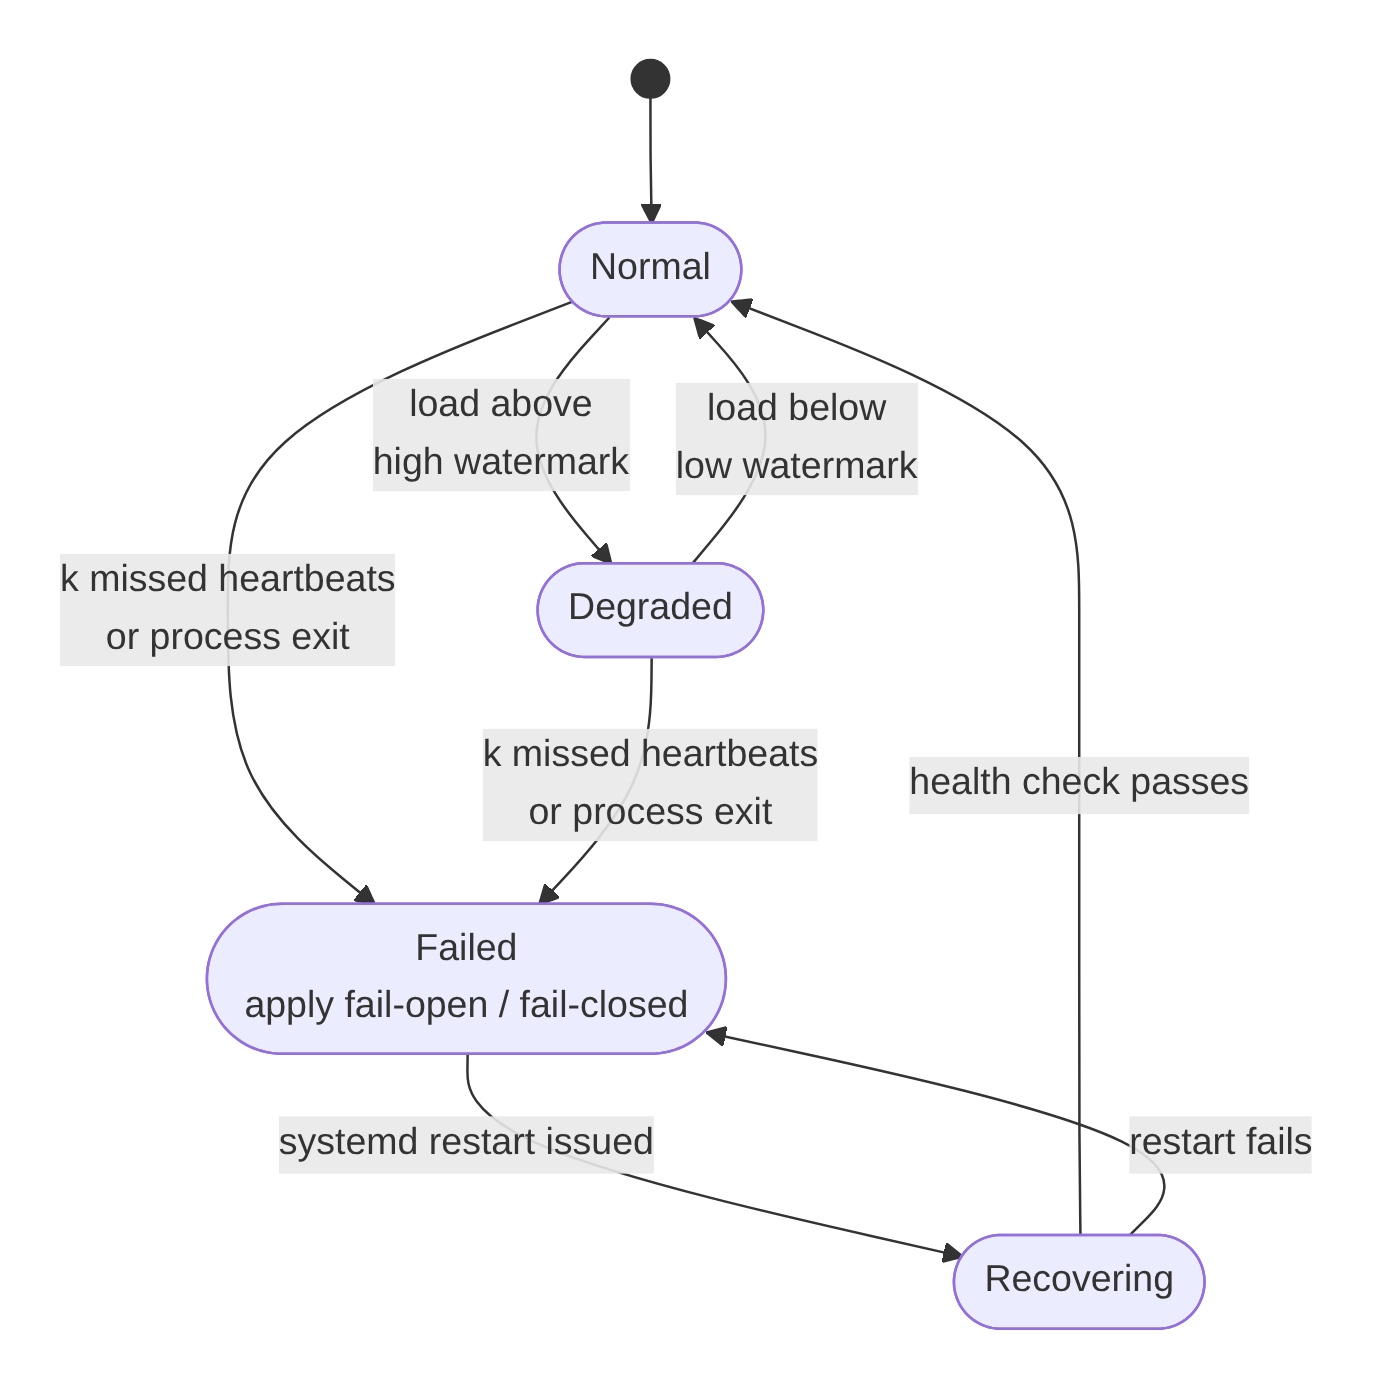
\includegraphics[width=0.55\textwidth]{Figures/nidps_fig5_3.png}
    \caption{Watchdog state machine for each supervised component.}
    \label{fig:statemachine}
\end{figure}

\noindent Two thresholds (high and low watermarks) are used for entering and leaving the degraded state. Without this gap, a load hovering around one value would cause the system to switch modes back and forth many times per second. During every failure, the watchdog records when it was detected, which mode was applied, when service resumed and how many packets were dropped or bypassed. These records produce the recovery measurements reported in the evaluation.

\section{Evaluation Methodology}\label{sec:5.10}
\label{sec:evaluation}
\noindent The system is evaluated on two questions: how well it detects attacks, and whether it can do so inline on constrained hardware without harming the network.

\subsection{Detection Metrics}\label{sec:5.10.1}
\label{sec:metrics}
\noindent For every layer and for the fused system, precision, recall, F1-score and false positive rate (FPR) are reported per class and macro-averaged:
\begin{equation}
\label{eq:metrics}
\begin{aligned}
\mathrm{Precision} &= \frac{TP}{TP + FP}, \qquad &
\mathrm{Recall} &= \frac{TP}{TP + FN}, \\
F_1 &= \frac{2 \cdot \mathrm{Precision} \cdot \mathrm{Recall}}{\mathrm{Precision} + \mathrm{Recall}}, \qquad &
\mathrm{FPR} &= \frac{FP}{FP + TN}
\end{aligned}
\end{equation}
\noindent False positive rate receives particular attention. On a home network producing thousands of flows per hour, even a 1\% false positive rate means dozens of wrong alerts or blocks every hour. For Layer 2, the area under the precision-recall curve is also reported, since it summarises performance across all thresholds and is more informative than ROC-AUC when attacks are rare.

\subsection{Cross-Dataset Generalisation}\label{sec:5.10.2}
\label{sec:crossdataset}
\noindent Each model is trained on one dataset and tested on every other dataset, giving the matrix in Table~\ref{tab:crossmatrix}. The diagonal (train and test on the same dataset, split by day) shows in-distribution performance. The off-diagonal cells show how much performance drops when the network changes, which is the realistic situation for a deployed device. Finally, models trained on all three public datasets combined are tested on the self-collected dataset.

\begin{table}[H]
\centering
\caption{Cross-dataset evaluation matrix of macro F1-scores, to be filled from experiments.}
\label{tab:crossmatrix}
\begin{tabular}{|>{\raggedright\arraybackslash}p{0.22\linewidth}|>{\raggedright\arraybackslash}p{0.14\linewidth}|>{\raggedright\arraybackslash}p{0.16\linewidth}|>{\raggedright\arraybackslash}p{0.14\linewidth}|>{\raggedright\arraybackslash}p{0.14\linewidth}|}
\hline
\textbf{Train / Test} & \textbf{CIC-IDS-2017} & \textbf{CSE-CIC-IDS2018} & \textbf{CIC-IoT-2023} & \textbf{Self-collected} \\
\hline
CIC-IDS-2017 & in-distribution & & & \\
\hline
CSE-CIC-IDS2018 & & in-distribution & & \\
\hline
CIC-IoT-2023 & & & in-distribution & \\
\hline
All three combined & & & & \\
\hline
\end{tabular}
\end{table}

\noindent Only classes that exist in both the training and the test dataset are scored in each cell. The adaptive threshold of Section~\ref{sec:calibration} is evaluated by comparing the false positive rate on the self-collected benign traffic with the global threshold and with the calibrated threshold.

\subsection{System Performance on Constrained Hardware}\label{sec:5.10.3}
\label{sec:sysperf}
\noindent Table~\ref{tab:sysperf} defines the system-level measures and how each is obtained.

\begin{table}[H]
\centering
\caption{System performance measures.}
\label{tab:sysperf}
\begin{tabular}{|>{\raggedright\arraybackslash}p{0.2\linewidth}|>{\raggedright\arraybackslash}p{0.3\linewidth}|>{\raggedright\arraybackslash}p{0.38\linewidth}|}
\hline
\textbf{Measure} & \textbf{Definition} & \textbf{How it is measured} \\
\hline
Forwarding latency & Extra round-trip time added by the NIDPS & Ping RTT through the AP with the NIDPS off, then with each layer enabled in turn \\
\hline
Throughput & Sustained forwarding rate & iperf3 TCP and UDP tests through the AP, layers enabled incrementally \\
\hline
Detection latency & Time from the first attack packet to the alert & Attack start logged on the attacker machine vs.\ alert timestamp \\
\hline
Time to block & Time from the first attack packet to the ipset entry & Same, against the audit record \\
\hline
Bytes leaked before block & Data the attacker transferred before the block took effect & Bytes received at the lab exfiltration server before the block, repeated at $T_a = 5$\,s and 10\,s \\
\hline
Resource use & CPU, memory and temperature of the host & Sampled every second during each test, at $T_a = 5$\,s and 10\,s \\
\hline
Recovery behaviour & Time to detect a failure, time to restore service, packets lost or bypassed & Components killed deliberately under load, in each failure mode \\
\hline
\end{tabular}
\end{table}

\noindent Every attack in the scope is replayed live against test devices on the isolated lab network while background benign traffic runs. This end-to-end test checks the complete chain, from detection through fusion to blocking, rather than each model in isolation.

\section{Conclusion}\label{sec:5.11}
\label{sec:ch5conclusion}
\noindent This chapter presented the proposed hybrid framework and the backend algorithms behind it. Suricata and an ARP consistency check provide fast, packet-level detection of known attacks. Isolation Forest, with a per-network threshold calibration, detects unusual behaviour, supported by host-level scores for exfiltration and C2 beaconing. A Random Forest or XGBoost classifier assigns flows to known attack families. Encrypted traffic is analysed through JA3/JA3S fingerprints and flow statistics instead of decryption, and all datasets are regenerated with the device's own flow extractor so training and runtime features match. A decision-fusion algorithm with host evidence accumulation turns these signals into verdicts, an enforcer applies them through timed ipset entries with safeguards against self-inflicted outages, and a watchdog applies a configurable failure mode backed by the kernel. The evaluation protocol measures both detection quality across datasets and the system's latency, throughput and recovery on real hardware. The next chapter describes how these algorithms are organised into components and how those components interact.
